\documentclass{article}
\usepackage[OT1]{fontenc} 
\usepackage[utf8]{inputenc}     
\usepackage[a4paper, left=0.8in, right=0.8in, top=1in,bottom=1in]{geometry}
\usepackage{graphicx}           
\usepackage{float}
\usepackage{subfigure} 
\usepackage{amsmath}    
\usepackage{amssymb}  
\usepackage{amsthm}
\usepackage{mathtools}         
\usepackage{enumitem}           
\usepackage{todonotes}          
\usepackage{newcent}            
\usepackage{hyperref}           
\usepackage[french]{babel}
\usepackage{listings} 
\usepackage{booktabs}\label{key}
\usepackage{setspace}

\renewcommand{\arraystretch}{1.7}
%%%%%%%%%%%%%%%%%%%%%%%
\newcommand\waveC{\underset{\approx}{C}}
\newcommand\WE[1]{W(\underset{=}{E}\large{\textcircled{\small{#1}}})}

\begin{document}
\begin{titlepage}
	\thispagestyle{empty}
	\newcommand{\HRule}{\rule{\linewidth}{0.5mm}}
	\center
	\textsc{\large ÉCOLE NATIONALE DES PONTS ET CHAUSSÉES}\\[.7cm]
	
\includegraphics[width=35mm]{ENPC_logo.png}\\[.5cm]
	\textsc{\large Département Génie Mécanique et Matériaux - 2019/2020}\\[0.5cm]
	
	\vspace{2cm}
	
	\HRule \\[0.4cm]
	{\LARGE {\fontfamily{pag}\selectfont { PROJET3 - Matériaux Hétérogènes }}\\
    \vspace{0.4cm}
	\HRule \\[.5cm]

\vspace{2cm}
\center
\large Réalisé par : {\fontfamily{pag}\selectfont{{\bfseries Andrey Latyshev} $\And$ {\bfseries Siyuan HE}  }}
\\
\vspace{1cm}
\center
Encadré par : 
\bfseries\fontfamily{pag}\selectfont{ {\bfseries Karam SAB}$\And${\bfseries Francis LAVERGNE} }

}
\end{titlepage}


\newpage
\begin{center}
    \tableofcontents
\end{center}


\newpage
\section{Préliminaires}\leavevmode \\
On considère un matériau cellulaire constitué d'une matrice élastique, linéaire et isotrope et de vide.Voici l'image pour montrer la géométrie de notre projet: 
\begin{figure}[h!]
    \begin{center}
    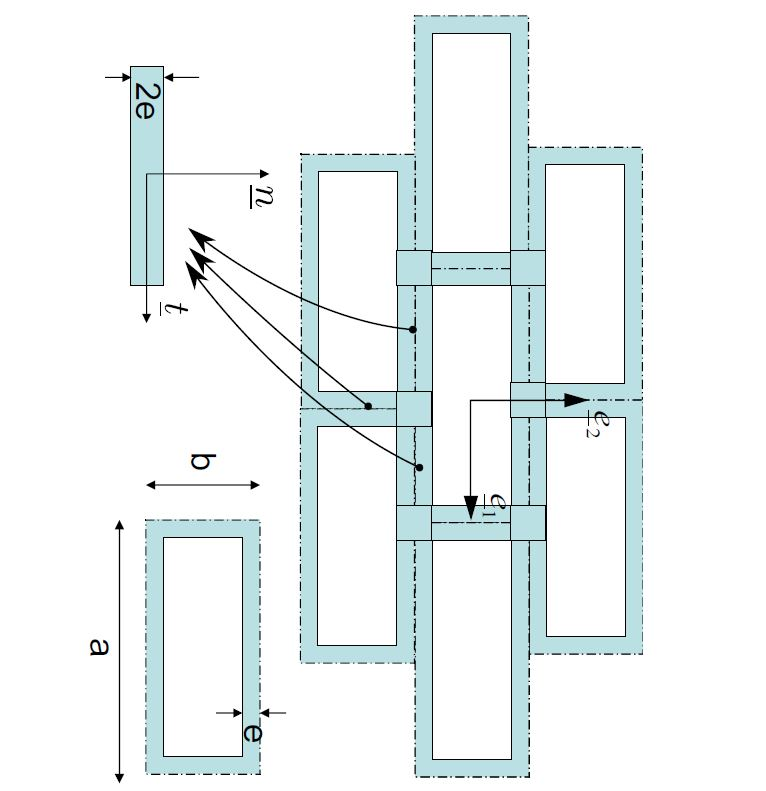
\includegraphics[width=8cm]{img/Géométrie_Projet3.JPG}
    \end{center}
    \caption{Géométrie du Projet3}
    \label{fig_géo générale}
\end{figure}
\par
L'hétérogénéité est invariant dans le sens 3. La répartition de la matière est périodique comme ci-dessus. Notre objectif est d'estimer numériquement le tenseur d'élasticité homogénéisé en déformation plane(1,2), $\waveC^{DP}=C^{DP}_{\alpha\beta\gamma\delta},\alpha,\beta,\gamma,\delta=1,2$, et de comparer cette estimation à une estimation théorique à construire. Le contrainte macroscopique et la déformation macroscopique n'a que les composantes en déformation plane (1,2). Le tenseur $\waveC^{DP}$ lie le contrainte macroscopique $\underset{\widetilde{}}{\Sigma}$ avec la déformation macroscopique $\underset{\widetilde{}}{E}$. On le écrit ci-dessous:\\
\begin{align*}
    \begin{pmatrix}
    \Sigma_{11}\\\Sigma_{22}\\2\Sigma_{12}
    \end{pmatrix} = 
    \begin{pmatrix}
    A & B & 0 \\ B & C & 0 \\ 0 & 0 & D
    \end{pmatrix}
    \begin{pmatrix}
    E_{11}\\E_{22}\\2E_{12}
    \end{pmatrix}
\end{align*}
Son énergie de déformation est: 
\begin{align*}
    W(\underline{E})={}& \frac{1}{2}\langle\underset{=}{ \varepsilon}:\waveC:\underset{=}{\varepsilon}\rangle
    \\
    ={}& \frac{1}{l_{1}l_{2}}\iint_{S}\frac{1}{2}\underset{=}{ \varepsilon}:\waveC:\underset{=}{\varepsilon}dS\\
    ={}& \frac{1}{2}(A E_{11}^{2}+2B E_{11}E_{22}+C E_{22}^{2}+4D E_{12}^{2})
\end{align*}



\section{Les problèmes plans de la détermination de $\underset{\approx}{C}^{DP}$}
Dans cette partie on essaie d'utiliser la périodicité et la symétrie du motif ci-dessus pour simplifier notre calculs. Il faut garder l'invariance de motif par rapport à la translation quelconque. D'abord on considère le cellule de base ci-dessous:
\begin{figure}[H]
    \begin{center}
    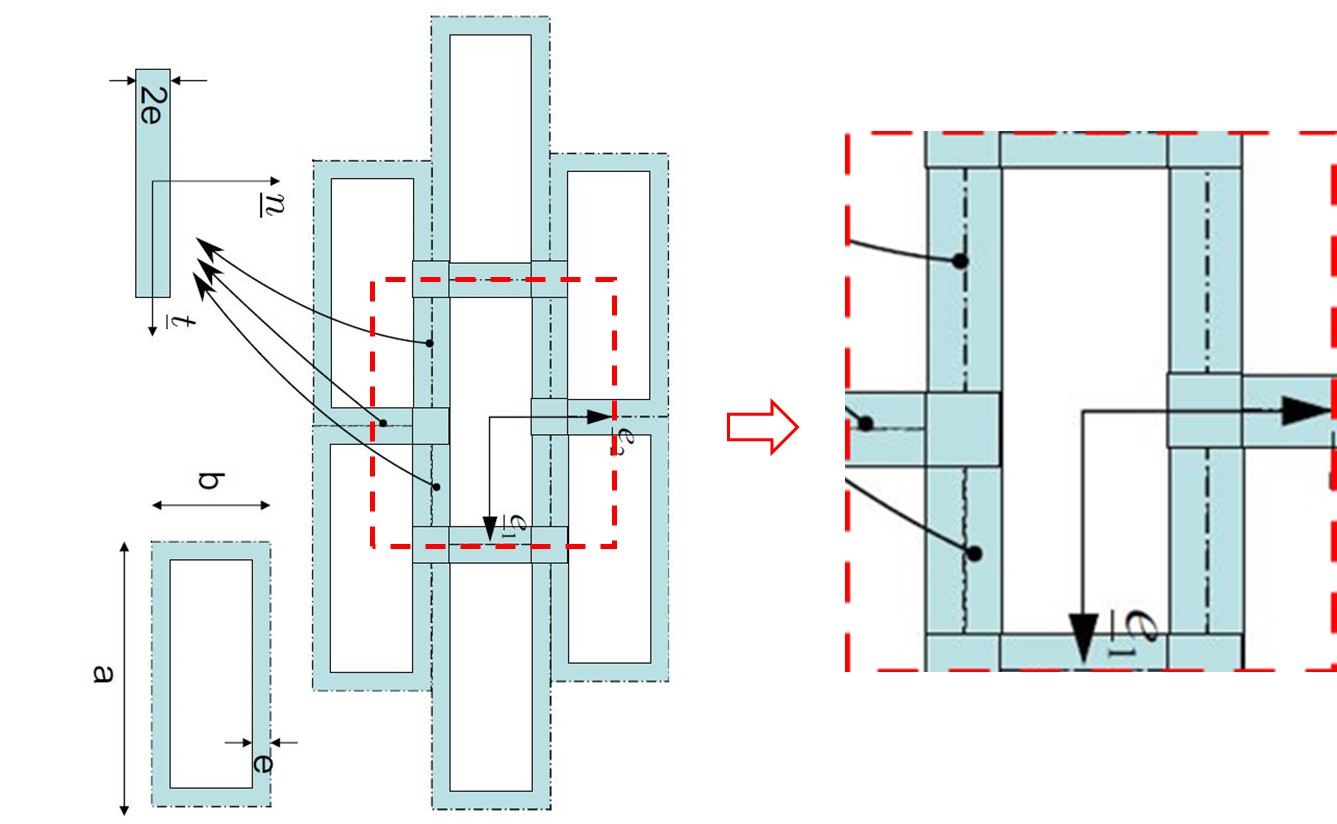
\includegraphics[width=6cm]{img/par_la_périodicité.JPG}
    \end{center}
    \caption{la première simplification par la périodicité}
    \label{fig_sim1}
\end{figure}
\par
En considérant la symétrie de cette profil, on a le droit de le simplifier encore. Il est centrosymétrique. On doit le couper par quatre morceaux et y ajouter les contraintes au bord sur le côté à gauche et sur le côté en haut. On précise le type des contraintes selon le chargement. Ensuite on obtient un cellule de base ci-dessous:\\ 
\begin{figure}[H]
    \begin{center}
    \includegraphics[width=6cm]{img/par_la_symétrie.jpg}
    \end{center}
    \caption{la deuxième simplification par la symétrie}
    \label{fig_sim2}
\end{figure}
\par
Rappelons l'expression de l'énergie, on veut déterminer les composantes de $\underset{\approx}{C}^{DP}$ séparément selon l'énergie totale mesurée par Abaqus ou bien estimée par la théorie de poutre. On élabore quatre cas de chargement:\\
\subsection{Essai \large{\textcircled{\small{1}}} - Détermination de A}
On fait un essai de la traction simple dans le sens 1: $\underset{=}{E}=\begin{pmatrix}E_{11} & 0\\ 0 & 0 \end{pmatrix}$. On impose $E_{11}=1$ et exprime le A en fonction de l'énergie totale correspondante:\\
\begin{align*}
    A=2W(\underset{=}{E}\large{\textcircled{\small{1}}})
\end{align*}
Pour les conditions aux limites, en considérant les simplifications par la périodicité et la symétrie, on fixe les liberté perpendiculaire aux côtés à gauche et en haut. 

\subsection{Essai \large{\textcircled{\small{2}}} - Détermination de C} 
On fait un essai de la traction simple dans le sens 2: $\underset{=}{E}=\begin{pmatrix}0 & 0\\ 0 & E_{22} \end{pmatrix} $. On impose $E_{22}=1$ et exprime le A en fonction de l'énergie totale correspondante:\\
\begin{align*}
    C=2W(\underset{=}{E}\large{\textcircled{\small{2}}})
\end{align*}
\par
Pour les conditions aux limites, en considérant les simplifications par la périodicité et la symétrie, on fixe les liberté perpendiculaire aux côtés à gauche et en haut. 

\subsection{Essai \large{\textcircled{\small{3}}} - Détermination de B}
On fait un essai de la traction en double sens 1 et 2:$\underset{=}{E}=\begin{pmatrix} E_{11} & 0\\ 0 & E_{22}\end{pmatrix}$. C'est-à-dire que l'on garde les trois termes A,B et C. On exprime le B en fonction de l'énergie totale correspondante avec A et C déterminées dans les essais avants:\\
\begin{align*}
    B=\frac{1}{2}(2W(\underset{=}{E}\large{\textcircled{\small{3}}})-A-C)
\end{align*}
Pour les conditions aux limites, en considérant les simplifications par la périodicité et la symétrie, on fixe les liberté perpendiculaire aux côtés à gauche et en haut. 

\subsection{Essai \large{\textcircled{\small{4}}} - Détermination de D}
On fait un essai du cisaillement simple: $\underset{=}{E}=\begin{pmatrix}0 & E_{12}\\E_{12}\end{pmatrix}$. On impose $E_{12}=\frac{1}{2}$ et exprime le D en fonction de l'énergie totale correspondante:\\
\begin{align*}
    D=2W(\underset{=}{E}\large{\textcircled{\small{4}}})
\end{align*}
Pour les conditions aux limites, en considérant les simplifications par la périodicité et la symétrie, on fixe les libertés coïncidentes avec les côtés à gauche et en haut. 



\section{Détermination numérique des composantes de $\underset{\approx}{C}^{DP}$}\leavevmode\\
On explique qu'est-ce que on a fait dans chaque partie de Abaqus.
\subsection{Géométrie}
\begin{figure}[h]
    \begin{minipage}[h]{0.49\linewidth}
        \center{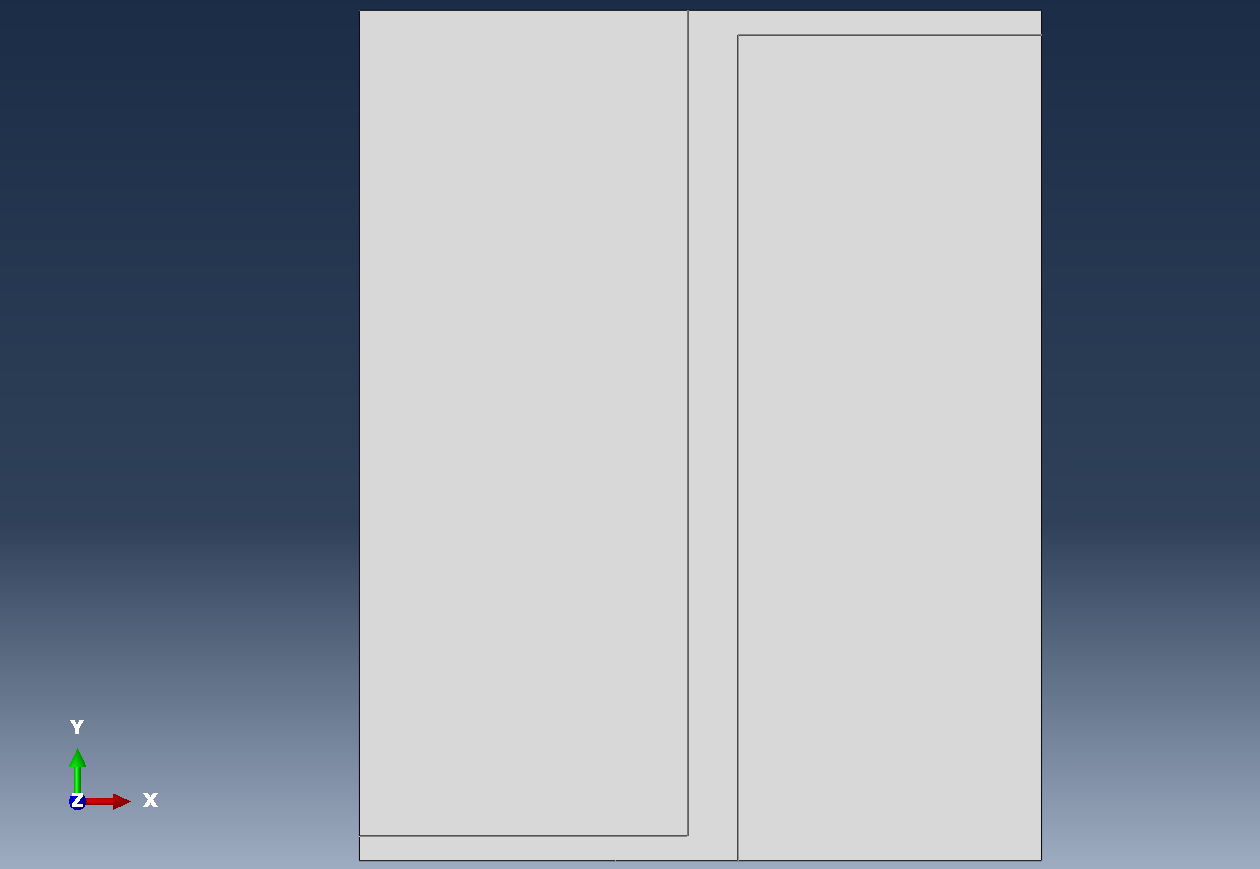
\includegraphics[width=1\linewidth]{img/Abaqus_geom1.png} }
    \end{minipage}
    \hfill
    \begin{minipage}[h]{0.49\linewidth}
        \center{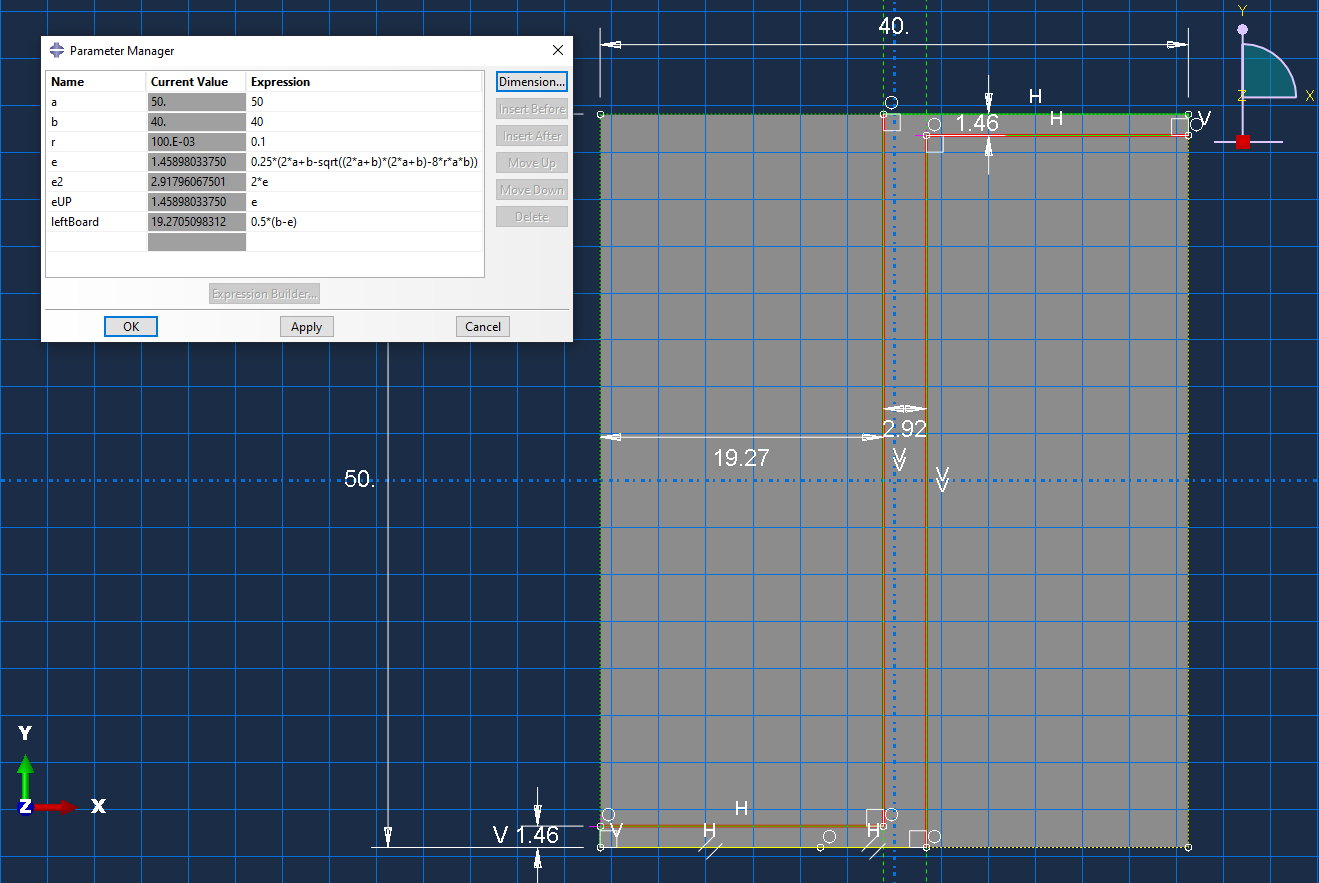
\includegraphics[width=1\linewidth]{img/Abaqus_geom2.png} }
    \end{minipage}
    \caption{La partie : Part}
\end{figure}

On a pris l'hauteur $a = 50$ et le longueur $b = 40$. Pour simplifier la variation de la quantité entre des volumes du "vide" et du matériau ( $r = \frac{ \text{superficie du matériau} }{ \text{superficie totale} }$ ), on utilise Parameter manager d'Abaqus.

\begin{align*}
    & r = \frac{2e(\frac{b}{2} + e) + 2e(a-2e)}{ab} \\
    & abr = -2e^2 + e(b + 2a) \\
    & e^2 - e \frac{b+2a}{2} + \frac{abr}{2} = 0 \\
    & e = \frac{2a + b - \sqrt{(2a+b)^2 - 8abr}}{4}
\end{align*}
Ici, on a pris en compte ce que $e < 2b < 2a$.

\subsection{Propriétés}
Notre structure contient deux matériaux élastiques : "l'acier abstrait" et "le vide". 
\begin{align*}
    & E_{acier} = 1, \quad \nu_{acier} = 0.3 \\
    & E_{vide} = 1^{-10}, \quad \nu_{vide} = 0.3
\end{align*}
Car $E_{vide}$ est presque null, donc cette partie ne influera pas sur le comportement du solid, mais très utile pour appliquer les conditions aux limites.
Pour l'avenir on aura besoin de 
\begin{equation*}
    E_s^{dp} = \frac{E_{acier}}{1-\nu_{acier}^2} = \frac{1}{1-0.09} \approx 1.1
\end{equation*}

\begin{figure}[H]
    \begin{minipage}[h]{0.49\linewidth}
        \center{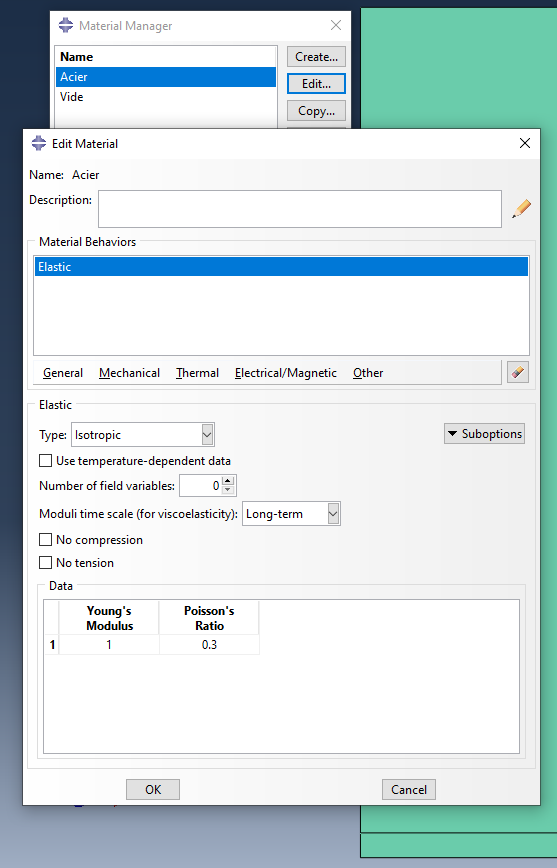
\includegraphics[width=0.8\linewidth]{img/Abaqus_mat1.png} }
    \end{minipage}
    \hfill
    \begin{minipage}[h]{0.49\linewidth}
        \center{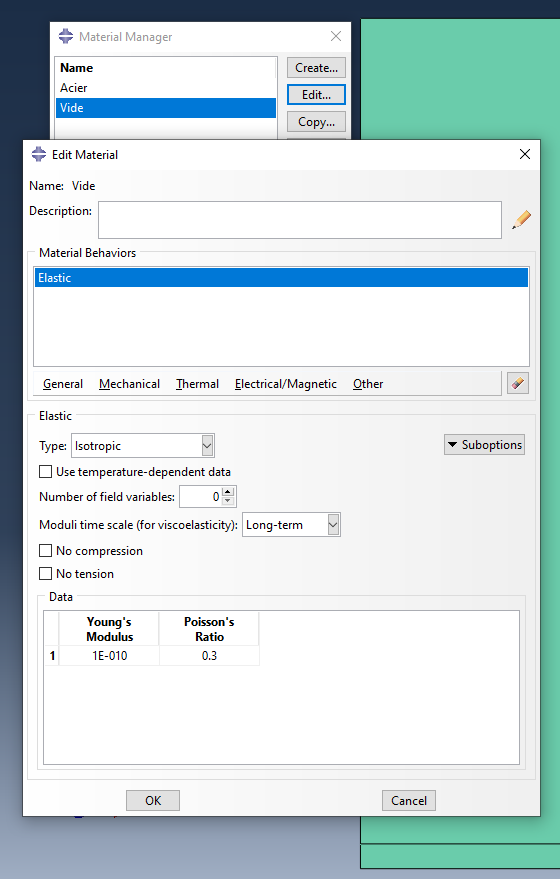
\includegraphics[width=0.8\linewidth]{img/Abaqus_mat2.png} }
    \end{minipage}
    \caption{La partie : Property}
\end{figure}
\par

\subsection{Conditions aux limites}
En prenant en compte des symétries de notre cellule, on peut appliquer les déplacements suivants 

\begin{figure}[H]
    \begin{minipage}[h]{0.47\linewidth}
        \center{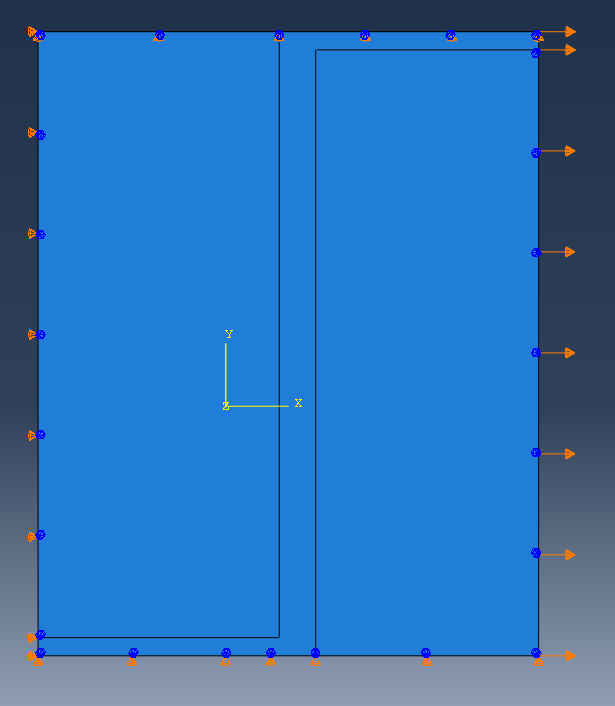
\includegraphics[width=1\linewidth]{img/Abaqus_CL_E11.png}} $E_{11}$ \\
    \end{minipage}
    \hfill
    \begin{minipage}[h]{0.47\linewidth}
        \center{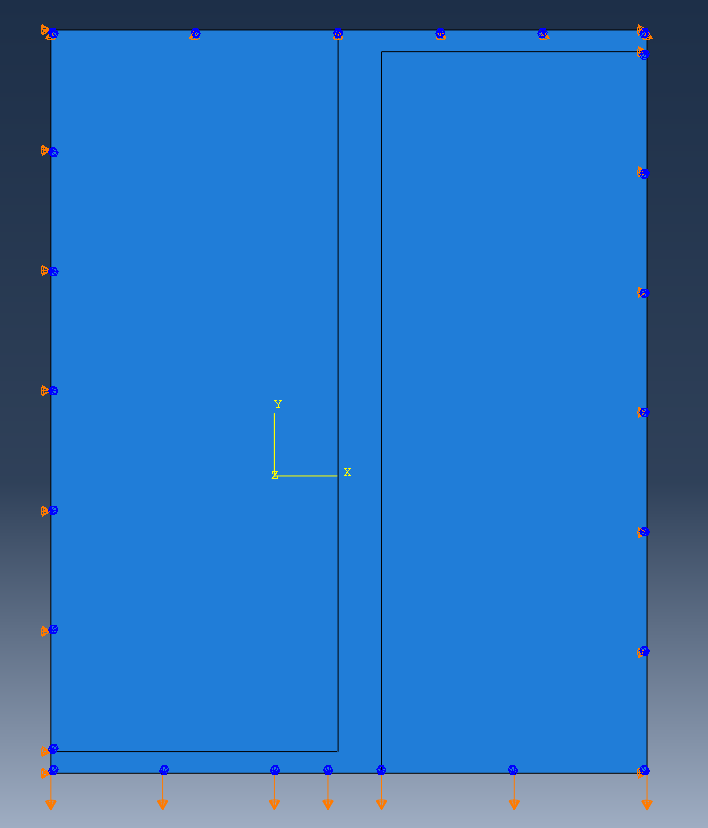
\includegraphics[width=1\linewidth]{img/Abaqus_CL_E22.png}} \\$E_{22}$
    \end{minipage}
    \vfill
    \begin{minipage}[h]{0.47\linewidth}
        \center{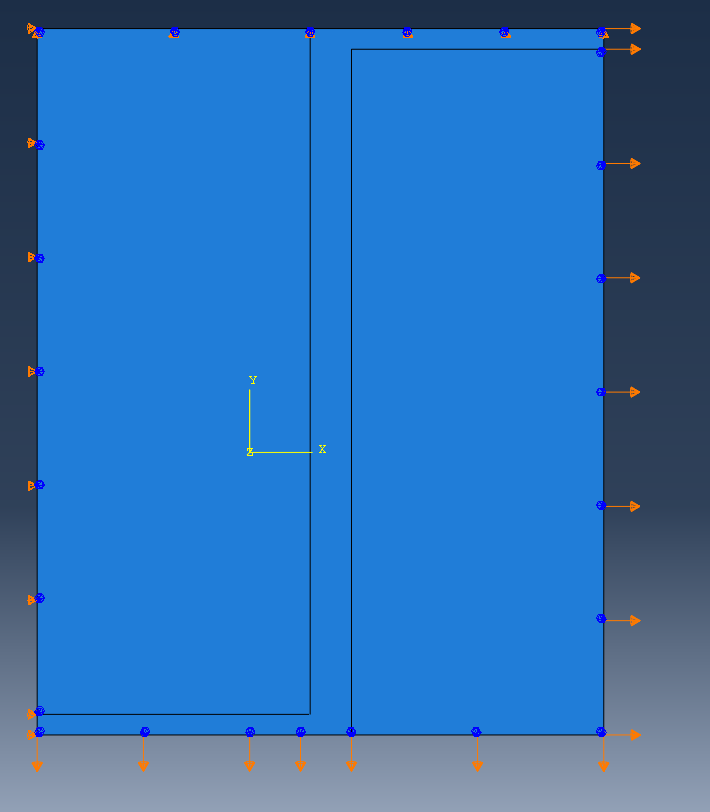
\includegraphics[width=1\linewidth]{img/Abaqus_CL_E11_E22.png}} $E_{11}+E_{22}$ \\
    \end{minipage}
    \hfill
    \begin{minipage}[h]{0.47\linewidth}
        \center{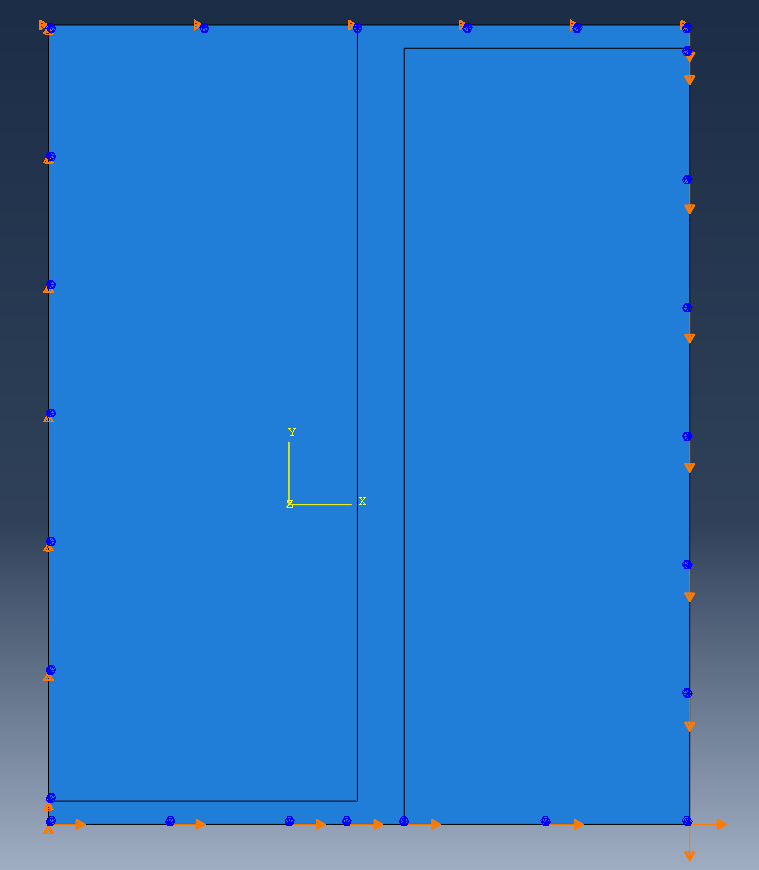
\includegraphics[width=1\linewidth]{img/Abaqus_CL_E12.png}} $E_{12}$ \\
    \end{minipage}
    \caption{La partie : Load}
\end{figure}


\begin{figure}[H]
    \begin{minipage}[h]{0.47\linewidth}
        \center{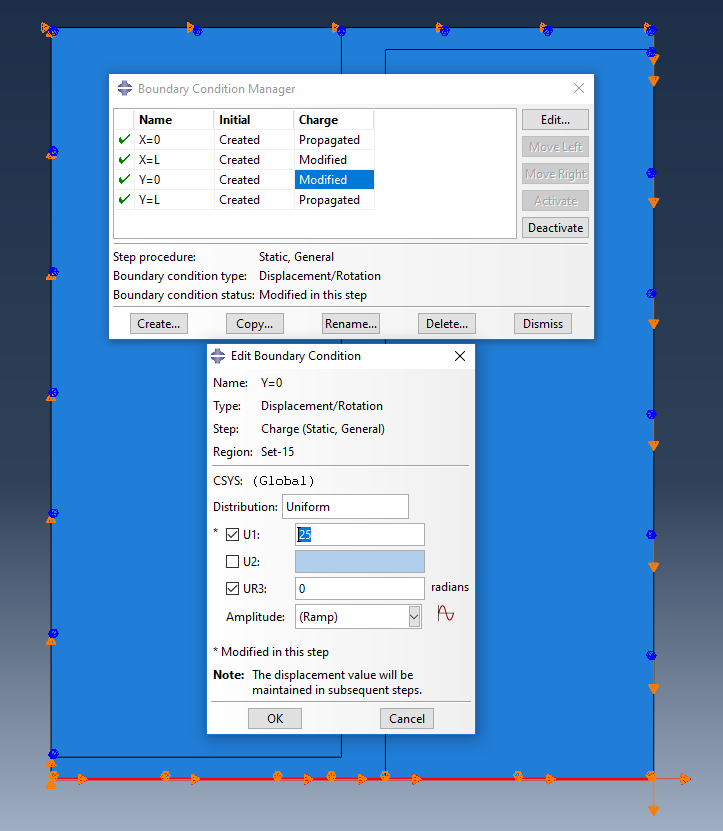
\includegraphics[width=1\linewidth]{img/Abaqus_disp1.png}} 
    \end{minipage}
    \hfill
    \begin{minipage}[h]{0.47\linewidth}
        \center{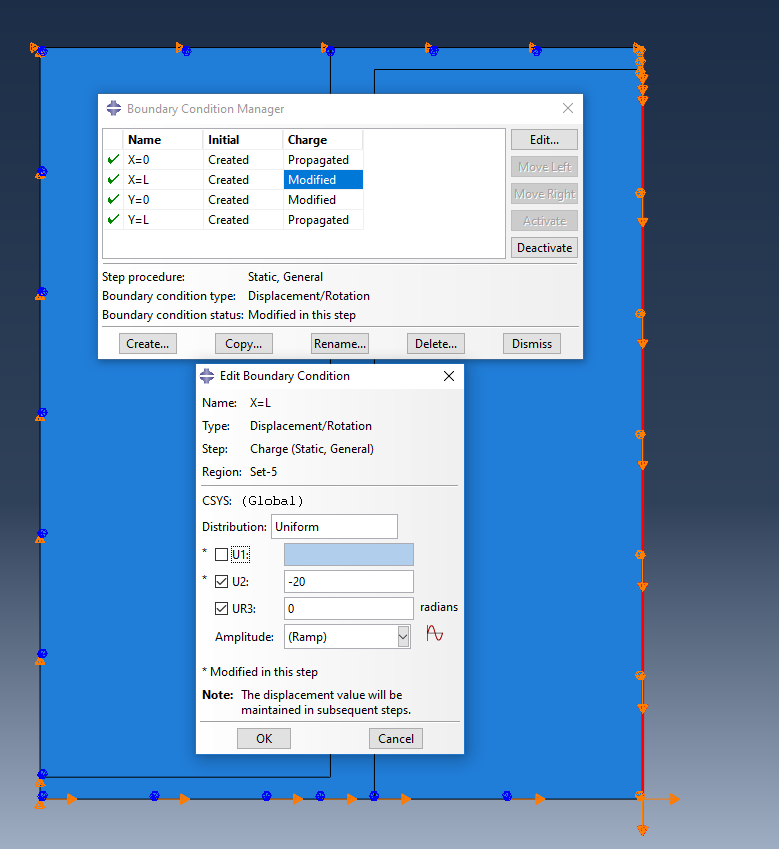
\includegraphics[width=1\linewidth]{img/Abaqus_disp2.png}}
    \end{minipage}
    \caption{La partie : Load. Les conditions aux limites pour le cas de cisaillement}
\end{figure}
On impose 
\begin{itemize}
    \item Cas $E_{11} : x = b$, \; $u_1 = E_{11}b = 1*40$
    \item Cas $E_{22} : y = 0$, \; $u_2 = -E_{22}a = -1*50$
    \item Cas $E_{11}+E_{22} : x = b$, \; $u_1 = E_{11}b = 1*40$; \quad $y = 0$, \; $u_2 = -E_{22}a = -1*50$
    \item Cas $E_{12} :x = b$, \; $u_2 = -E_{12}b = \frac{1}{2}*40 = 20$; \quad $y = 0$, \; $u_1 = E_{12}a = \frac{1}{2}*50 = 25$
\end{itemize}

\subsection{Maillage}
On résout le problème Plane strain, donc on peut prendre des paramètres du maillage suivants

\begin{figure}[H]
    \begin{minipage}[h]{0.4\linewidth}
        \center{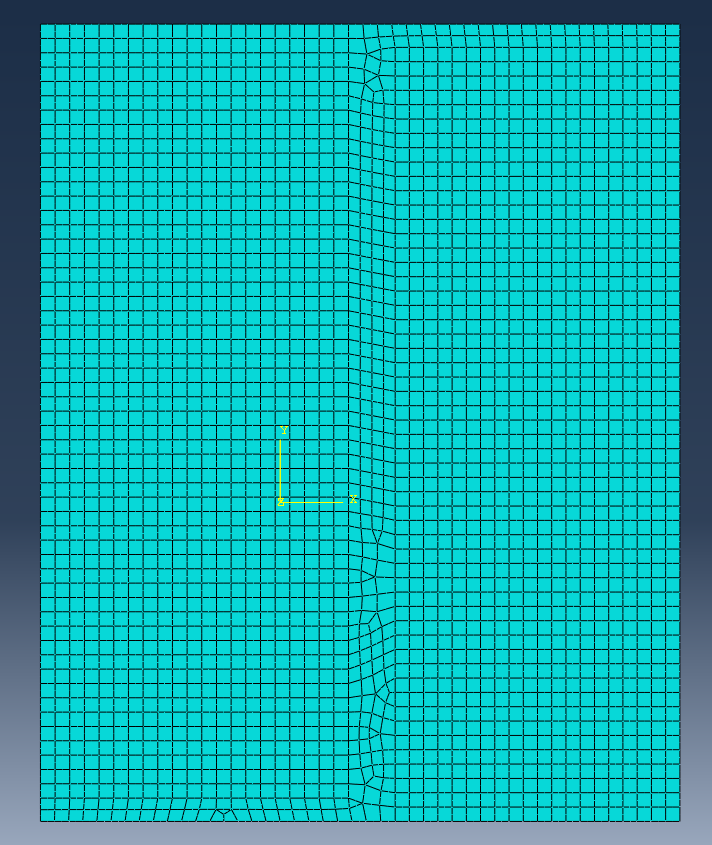
\includegraphics[width=1\linewidth]{img/Abaqus_mesh1.png}} \\
    \end{minipage}
    \hfill
    \begin{minipage}[h]{0.4\linewidth}
        \center{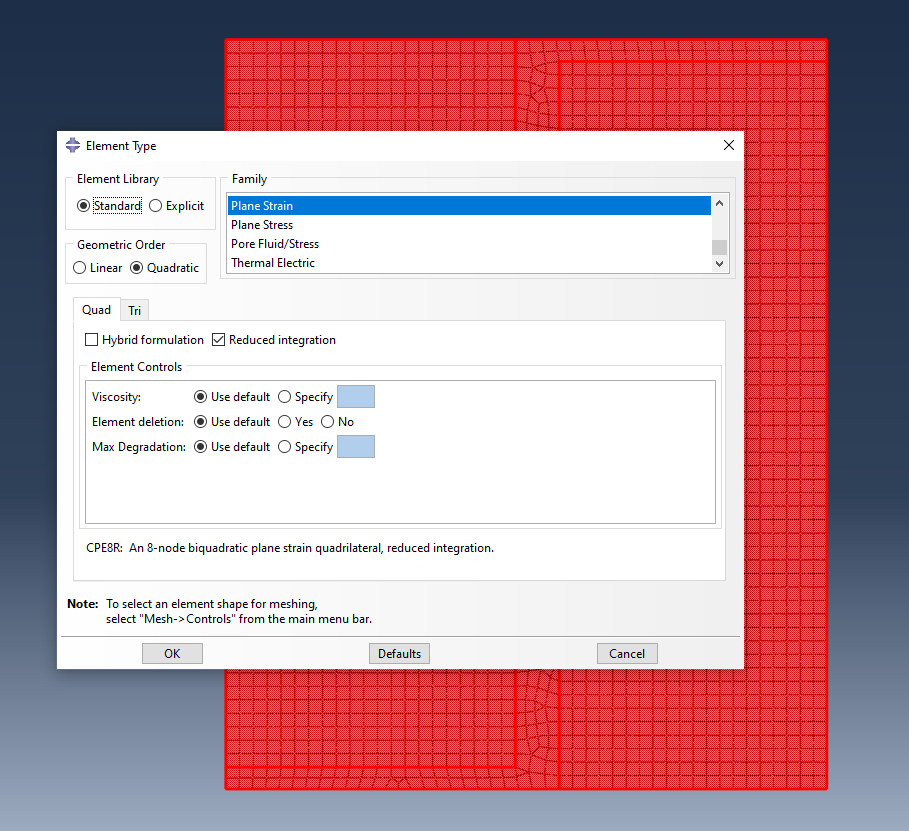
\includegraphics[width=1\linewidth]{img/Abaqus_mesh2.png}} \\
    \end{minipage}
    \caption{La partie : Mesh}
\end{figure}

\subsection{Résultats de la modélisation}

En résultat, on a calculé l'énergie élastique du solide pour 5 cas différents de la relation entre les quantités des matériaux et il y a respectivement quatre énergies pour quatre types des chargements.
\begin{table}[H]
    \begin{tabular}{|r|r|r|r|r|r|}
        \hline
        r & 0.1         & 0.05        & 0.03         & 0.02         & 0.01          \\ \hline
        e & 1.458980338 & 0.721726998 & 0.4312279651 & 0.2868900846 & 0.1431498841  \\ \hline
        $W(\underset{=}{E}\large{\textcircled{\small{1}}})$ & 0.180153    & 0.0215743   & 0.00444592   & 0.0012557    & 0.000158278   \\ \hline
        $W(\underset{=}{E}\large{\textcircled{\small{2}}})$ & 80.4211     & 39.7397     & 23.7238      & 15.761       & 7.86863       \\ \hline
        $W(\underset{=}{E}\large{\textcircled{\small{3}}})$ & 80.7134     & 39.7748     & 23.7312      & 15.7642      & 7.86911       \\ \hline
        $W(\underset{=}{E}\large{\textcircled{\small{4}}})$ & 0.112192    & 0.01320525  & 0.002795175  & 0.000823555  & 0.00009979875 \\ \hline
        $A(\waveC_{1111}^{DP})$ & 0.360306    & 0.0431486   & 0.00889184   & 0.0025114    & 0.000316556   \\ \hline
        $B(\waveC^{DP}_{1122})$ & 0.112147    & 0.0135257   & 0.00295408   & 0.0019443    & 0.000321722   \\ \hline
        $C(\waveC^{DP}_{2222})$ & 160.8422    & 79.4794     & 47.4476      & 31.522       & 15.73726      \\ \hline
        $D(\waveC^{DP}_{1212})$ & 0.224384    & 0.0264105   & 0.00559035   & 0.00164711   & 0.0001995975  \\ \hline
    \end{tabular}
    \caption{L'énergie élastique et composantes $C_{ijkl}$ calculés par Abaqus}
\end{table}

\begin{table}[H]
    \begin{tabular}{|r|r|r|r|r|r|}
    \hline
        $\log_{10}(r)$ & -1            & -1.301029996 & -1.522878745 & -1.698970004 & -2           \\ \hline
        $\log_{10}(A)$ & -0.4433285057 & -1.365033291 & -2.051008361 & -2.60008411  & -3.49954945  \\ \hline
        $\log_{10}(B)$ & -0.9502123396 & -1.868840249 & -2.529577748 & -2.711236724 & -3.49251924  \\ \hline
        $\log_{10}(C)$ & 2.206400005   & 1.90025458   & 1.67621425   & 1.498613765  & 1.19692912   \\ \hline
        $\log_{10}(D)$ & -0.6490081143 & -1.578223377 & -2.252561001 & -2.783277396 & -3.699844903 \\ \hline
    \end{tabular}
    \caption{Les valeurs des logarithmes}
\end{table}

\begin{figure}[H]
    \begin{center}
        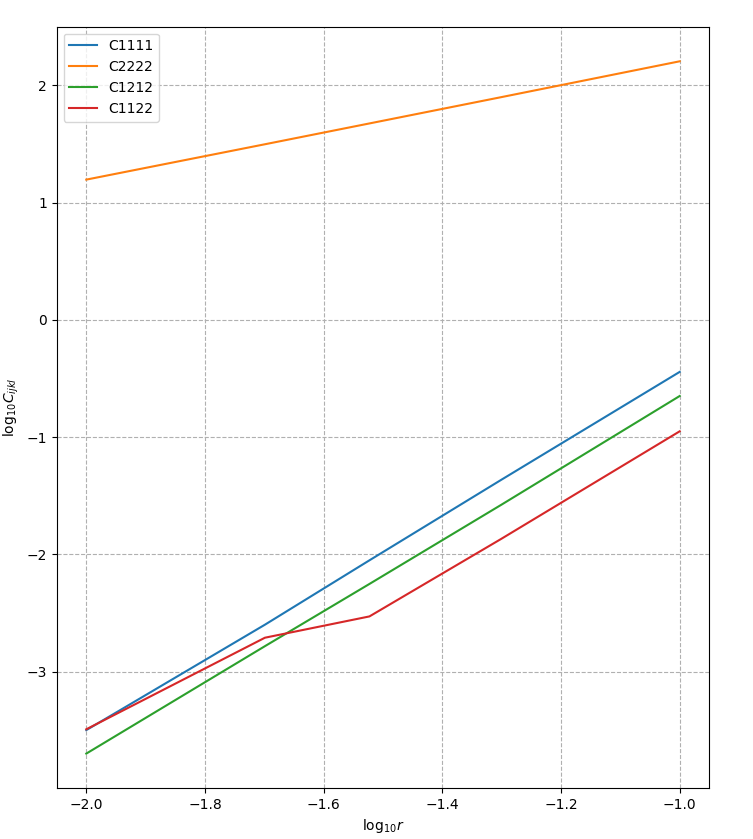
\includegraphics[width=0.8\linewidth]{img/Abaqus_CDP1.png}
    \end{center}
    \caption{La dépendance logarithmique de $r$}
\end{figure}

On peut exprimer le loi de cette dépendance. Soit

\begin{align*}
    & \log_{10}(C_{ijkl}) = k * \log_{10}(r) + h \\
    & C_{ijkl} = const * r^k
\end{align*}

\begin{table}[H]
    \begin{tabular}{|r|r|r|r|r|r|}
        \hline
         & & & & & Médian \\ \hline
        $k_A$                       & 3.061837021 & 3.092084454 & 3.118131771   & 2.987959185 & 3.065003108 $\approx$ 3 \\ \hline
        $k_B$                      & 3.051615863 & 2.978324193 & 1.031618362   & 2.595364341 & 2.41423069 $\approx$ 2.4\\ \hline
        $k_C$                       & 1.016993088 & 1.009878715 & 1.008570704   & 1.002174697 & 1.009404301 $\approx$ 1\\ \hline
        $k_D$                      & 3.086786287 & 3.039627789 & 3.013871318   & 3.044771351 & 3.046264186 $\approx$ 3\\ \hline
    \end{tabular}
\end{table}
Ainsi,

\begin{align}
\label{eqn:Cijkl_num}
    & C_{1111} = const * r^3 \\
    & C_{1122} = const * r^{2.4} \\
    & C_{2222} = const * r \\
    & C_{1212} = const * r^3 
\end{align}

\section{Estimation théorique de $\underset{\approx}{C}^{DP}$}\leavevmode\\
On décompose le cellule de base en trois poutres, et on estime ses énergies par la théorie des poutres en flexion cylindrique. selon cette théorie, l'énergie par unité de longueur dans le sens 3 d'une "poutre" droite de longueur $L$ et d'épaisseur $h$ est égale à:\\
\begin{align*}
    \frac{1}{2}E_{s}^{dp}(\frac{h}{L}(u^{+}-u^{-})^{2}+\frac{h^{3}}{L^{3}}(\nu^{+}-\nu^{-}+L\frac{\varphi^{+}+\varphi^{-}}{2})^{2}+\frac{h^{3}}{12L}(\varphi^{+}-\varphi^{-})^{2})
\end{align*}
Où $E_{s}^{dp}=\frac{E_{s}}{1-\nu^{2}}$ et $(u^{+},\nu^{+},\varphi^{+})(u^{-},\nu^{-},\varphi^{-})$ sont les libertés de deux extrémités du poutre en déformation plane. Les deux blocs sont différents en topologie donc on le nomme comme noeud type 1 et noeud type 2.Voici un schéma ci-dessous:\\
\begin{figure}[H]
    \begin{center}
    \includegraphics[width=8cm]{img/répartition.jpg}
    \end{center}
    \caption{Répartition du cellule de base}
    \label{fig_répartition}
\end{figure}
\begin{figure}[H]
    \begin{center}
    \includegraphics[width=8cm]{img/liberté.jpg}
    \end{center}
    \caption{Libertés correspondant aux poutres}
    \label{fig_liberté}
\end{figure}
\par
Les énergies dans les deux petits blocs sont négligeables par rapport à la dimension du cellule. Mais on vas utiliser les déplacements en bout du poutre pour exprimer l'énergie du système. On regarde les libertés comme les variables dans la minimisation de l'énergie élastique totale. Selon le "Principe d'énergie potentielle minimale", le champs de déplacement correspondant à l'énergie minimale est cinématiquement admissible. Il reste alors à trouver un moyen de déterminer des composantes de $\xi$. On utilise alors la relation:\\
\begin{align*}
    \underline{\xi}&=\underset{=}{E}\cdot\underset{-}{y}+\underline{\xi_{per}}\\
    CA(\underset{=}{E})&=\bigl\{\xi,\xi(\underline{y})=\underset{=}{E}\cdot\underline{y}+\underline{\xi_{per}}(\underline{y}),\text{ $\underline{\xi_{per}}$ périodique sur $\partial Y$} \bigr\}
\end{align*}
avec
\begin{align*}
    \underline{\xi_{per}}={}& \underline{\xi_{per}^{1}}\text{ sur les blocs de type 1} \\
    \underline{\xi_{per}}={}& \underline{\xi_{per}^{2}}\text{ sur les blocs de type 2} 
\end{align*}

\subsection{Essai \large{\textcircled{\small{1}}}}
Au vu de la déformation considérée (traction selon e1), nous avons : $\varphi_{0}=\varphi_{1}=\varphi_{2}=\varphi_{3}=0$\\
\begin{align*}
    \underset{=}{E}=\begin{pmatrix}E_{11}&0\\0&0\end{pmatrix}
\end{align*}
Condition au limite en bas : $\xi_{2}(x_{2}=0)=0$ \\
Maintenant on arrive au niveau d'un noeud de type 1:\\
\begin{align*}
    \underline{\xi}(x_{1}=\frac{b}{2},x_{2}=0)=\begin{pmatrix}E_{11}&0\\0&0\end{pmatrix}\cdot\begin{pmatrix}\frac{b}{2}\\0\end{pmatrix}+\underline{\xi}_{per}^{1}
\end{align*}
On en déduit que: $\xi_{per,2}^{1}=0$\\
Condition au limite en haut : $\xi_{2}(x_{2}=a)=0$ \\
Maintenant on arrive au niveau d’un noeud de type 2 :\\
\begin{align*}
    \underline{\xi}(x_{1}=\frac{b}{2},x_{2}=a)=\begin{pmatrix}E_{11}&0\\0&0\end{pmatrix}\cdot\begin{pmatrix}\frac{b}{2}\\a\end{pmatrix}+\underline{\xi}_{per}^{2}
\end{align*}
On en déduit que: $\xi_{per,2}^{2}=0$\\
Alors on exprime l’énergie élastique en fonction de $\xi_{per,1}^{1}=0$ et $\xi_{per,1}^{2}=0$:\\
\begin{align*}
    W=\frac{1}{2}\frac{E_{s}}{1-\nu_{s}^{2}}(\frac{e}{\frac{b}{2}-e}(E_{11}\frac{b}{2}+\xi_{per,1}^{1}-0)^{2})+\frac{1}{2}\frac{E_{s}}{1-\nu_{s}^{2}}((\frac{2e}{a-2e})^{3}(\xi_{per,1}^{1}-\xi_{per,1}^{2})^{2})+\frac{1}{2}\frac{E_{s}}{1-\nu_{s}^{2}}(\frac{e}{\frac{b}{2}-e}(E_{11}\frac{b}{2}+\xi_{per,1}^{2}-E_{11}b)^{2})
\end{align*}
La valeur minimale se trouve seulement dans cette condition:\\
\begin{align*}
    \xi_{per,1}^{1}&=-E_{11}\frac{b}{2}\\
    \xi_{per,1}^{2}&=E_{11}\frac{b}{2}\\
\end{align*}
L'énergie élastique cinématique admissible:\\
\begin{align*}
    W=\frac{1}{2}\frac{E_{s}}{1-\nu_{s}^{2}}((\frac{2e}{a-2e})^{3}(E_{11}b)^{2})
\end{align*}

\subsection{Essai \large{\textcircled{\small{2}}}}
Au vu de la déformation considérée (traction selon e2), nous avons : $\varphi_{0}=\varphi_{1}=\varphi_{2}=\varphi_{3}=0$\\
\begin{align*}
    \underset{=}{E}=\begin{pmatrix}0&0\\0&E_{22}\end{pmatrix}
\end{align*}
Condition au limite en bas : $\xi_{2}(x_{2}=0)=-E_{22}$ \\
Maintenant on arrive au niveau d'un noeud de type 1:\\
\begin{align*}
    \underline{\xi}(x_{1}=\frac{b}{2},x_{2}=0)=\begin{pmatrix}0&0\\0&E_{22}\end{pmatrix}\cdot\begin{pmatrix}\frac{b}{2}\\0\end{pmatrix}+\underline{\xi}_{per}^{1}
\end{align*}
On en déduit que: $\xi_{per,2}^{1}=-E_{22}a$\\
Condition au limite en haut : $\xi_{2}(x_{2}=a)=0$ \\
Maintenant on arrive au niveau d’un noeud de type 2 :\\
\begin{align*}
    \underline{\xi}(x_{1}=\frac{b}{2},x_{2}=a)=\begin{pmatrix}0&0\\0&E_{22}\end{pmatrix}\cdot\begin{pmatrix}\frac{b}{2}\\a\end{pmatrix}+\underline{\xi}_{per}^{2}
\end{align*}
On en déduit que: $\xi_{per,2}^{2}=-E_{22}a$\\
Alors on exprime l’énergie élastique en fonction de $\xi_{per,1}^{1}=0$ et $\xi_{per,1}^{2}=0$:\\
\begin{align*}
    W=\frac{1}{2}\frac{E_{s}}{1-\nu_{s}^{2}}(\frac{e}{\frac{b}{2}-e}(\xi_{per,1}^{1})^{2})+\frac{1}{2}\frac{E_{s}}{1-\nu_{s}^{2}}(\frac{2e}{a-2e}(E_{22}a)^{2}+(\frac{2e}{a-2e})^{3}(\xi_{per,1}^{1}-\xi_{per,1}^{2})^{2})+\frac{1}{2}\frac{E_{s}}{1-\nu_{s}^{2}}(\frac{e}{\frac{b}{2}-e}(\xi_{per,1}^{2})^{2})
\end{align*}
La valeur minimale se trouve seulement dans cette condition:\\
\begin{align*}
    \xi_{per,1}^{1}=\xi_{per,1}^{2}=0
\end{align*}
L'énergie élastique cinématique admissible:\\
\begin{align*}
    W=\frac{1}{2}\frac{E_{s}}{1-\nu_{s}^{2}}(\frac{2e}{a-2e}(E_{22}a)^{2})
\end{align*}

\subsection{Essai \large{\textcircled{\small{3}}}}
Au vu de la déformation considérée (traction selon e1 et e2), nous avons : $\varphi_{0}=\varphi_{1}=\varphi_{2}=\varphi_{3}=0$\\
\begin{align*}
    \underset{=}{E}=\begin{pmatrix}E_{11}&0\\0&E_{22}\end{pmatrix}
\end{align*}
L'énergie élastique cinématique admissible:\\
\begin{align*}
    W=\frac{1}{2}\frac{E_{s}}{1-\nu_{s}^{2}}((\frac{2e}{a-2e})^{3}(E_{11}b)^{2})+\frac{1}{2}\frac{E_{s}}{1-\nu_{s}^{2}}(\frac{2e}{a-2e}(E_{22}a)^{2})
\end{align*}

\subsection{Essai \large{\textcircled{\small{4}}}}
\subsubsection{façon 1}
\begin{figure}[H]
    \begin{center}
    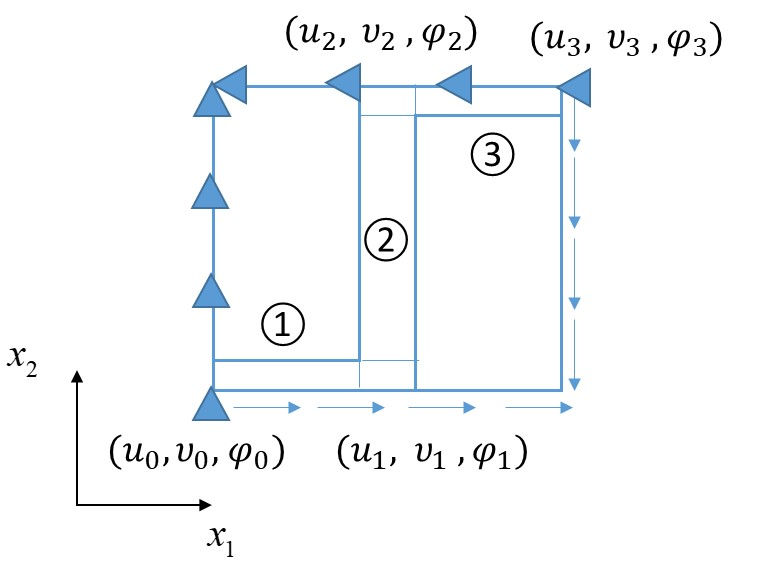
\includegraphics[width=8cm]{img/cisaillement.jpg}
    \end{center}
    \caption{Les conditions aux limites}
    \label{fig_cisaillement}
\end{figure}
\par
Apparemment il n’y pas de compression ni de traction dans le poutre \large{\textcircled{\small{3}}}. Selon l’anti-symétrie, le poutre \large{\textcircled{\small{1}}} est pareil, ainsi donc le premier terme de l’énergie élastique totale est nulle. En raison du cisaillement simple, tous les déplacements ver la direction 1 sont nuls. Selon la symétrie par rapport au côté en haut, le $\varphi_{2}=0$. Selon la périodicité, le bord déformé doit coïncide. On en déduit que $\varphi_{1}=0$. Selon l’anti-symétrie, la rotation du poutre \large{\textcircled{\small{1}}} et celle-ci du \large{\textcircled{\small{3}}} sont pareils. On impose $\varphi_{3}=\varphi_{0}=\phi$.\\
Le déplacement des quatre extrémités s’écrit comme:
\begin{align*}
    (u_{0},\nu_{0},\phi_{0})&=(0,0,\phi)\\
    (u_{1},\nu_{1},\phi_{1})&=(0,\nu_{1},0)\\
    (u_{2},\nu_{2},\phi_{2})&=(0,\nu_{2},0)\\
    (u_{3},\nu_{3},\phi_{3})&=(0,E_{12}b,\phi)
\end{align*}
Pour le poutre \large{\textcircled{\small{1}}}, l’énergie élastique s’écrit comme ci-dessous:\\
\begin{align*}
    W_{1}&=\frac{1}{2}E_{s}^{dp}(\frac{h^{3}}{L^{3}}(0-\nu_{1}+L\frac{\phi}{2})^{2}+\frac{h^{3}}{12L}\phi^{2})\\
    h&=e\\
    L&=\frac{b}{2}-e
\end{align*}
Pour le poutre \large{\textcircled{\small{3}}}, l’énergie élastique s’écrit comme ci-dessous:\\
\begin{align*}
    W_{3}&=\frac{1}{2}E_{s}^{dp}(\frac{h^{3}}{L^{3}}(\nu_{2}-E_{12}\cdot b+L\frac{\phi}{2})^{2}+\frac{h^{3}}{12L}\phi^{2})\\
    h&=e\\
    L&=\frac{b}{2}-e
\end{align*}
Pour le poutre \large{\textcircled{\small{2}}}, l’énergie élastique s’écrit comme ci-dessous:\\
\begin{align*}
    W_{2}&=\frac{1}{2}E_{s}^{dp}(\frac{h}{L}(\nu_{1}-\nu_{2})^{2})\\
    h&=2e\\
    L&=a-2e
\end{align*}
Finalement on obtient l’énergie élastique totale:\\
\begin{align*}
    W=W_{1}+W_{2}+W_{3}
\end{align*}
On utilise le logiciel Wolfram Mathematica pour minimiser cette fonction par rapport aux variables $\phi$, $\nu_{1}$, et $\nu_{2}$. On précise les paramètres géométriques et montre les résultats trouvés dans la dernière section.
\subsubsection{façon 2}
\begin{figure}[H]
    \begin{center}
    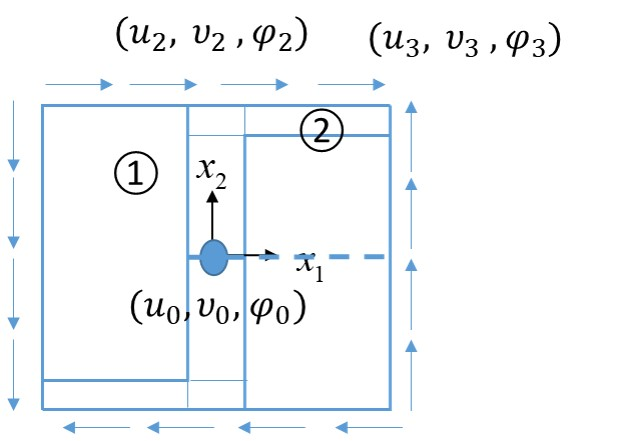
\includegraphics[width=8cm]{img/cisaillement2.jpg}
    \end{center}
    \caption{Les conditions aux limites}
    \label{fig_cisaillement}
\end{figure}
\par
\begin{align*}
    (u_{0},\nu_{0},\phi_{0})&=(0,0,\phi_0)\\
    (u_{2},\nu_{2},\phi_{2})&=(E_{12}\frac{a}{2},\nu_{2},\phi_2)\\
    (u_{3},\nu_{3},\phi_{3})&=(E_{12}\frac{a}{2},E_{12}\frac{b}{2},\phi_3)
\end{align*}
\begin{align*}
    W_{1}&=\frac12 E_s^{dp} \left(\frac{h}{L}(\nu_2)^2+
        \frac{h^3}{L^3}\left( - E_{12}\frac{a}{2} +
        L\frac{\phi_0+\phi_2}{2} \right)^2 + \frac{h^3}{12L}(\phi_0-\phi_2)^2 \right)\\
    h&=2e\\
    L&=\frac{a}{2}-e
\end{align*}
\begin{align*}
    W_{2}&=\frac12 E_s^{dp} \left(
        \frac{h^3}{L^3}\left( E_{12}\frac{b}{2}-\nu_2 +
        L\frac{\phi_2+\phi_3}{2} \right)^2 + \frac{h^3}{12L}(\phi_2-\phi_3)^2 \right)\\
    h&=e\\
    L&=\frac{b}{2}-e
\end{align*}
\begin{align*}
    W=2*(W_{1}+W_{2})
\end{align*}

\par

\section{Comparaison et synthèse}\leavevmode \\
L'application de ces formules nous donne l'approximation théorétique des valeurs d'énergie.

\begin{table}[H]
    \begin{tabular}{|r|r|r|r|r|r|}
    \hline
    r  & 0.1       & 0.05 & 0.03        & 0.02        & 0.01                                                                         \\ \hline
    $\WE{1}_{theorie}$ & 0.209277  & 0.0230948  & 0.00475356  & 0.00137535  & 0.000167913 \\ \hline
    $\WE{2}_{theorie}$ & 85.132    & 40.8342 & 24.1097     & 15.9462     & 7.91067                 \\ \hline
    $\WE{3}_{theorie}$ & 85.341277 & 40.8572948 & 24.11445356 & 15.94757535 & 7.910837913     \\ \hline
    $\WE{4}_{theorie}$                & 0.0133727 & 0.00144118 & 0.000293965 & 0.000084677 & 0.0000102929          \\ \hline
    $A_{theorie}$  & 0.418554  & 0.0461896 & 0.00950712  & 0.0027507   & 0.000335826                                         \\ \hline
    $B_{theorie}$ & 0         & 0 & 0           & 0           & 0                            \\ \hline
    $C_{theorie}$ & 170.264   & 81.6684   & 48.2194     & 31.8924     & 15.82134                     \\ \hline
    $D_{theorie}$ & 0.0267454 & 0.00288236 & 0.00058793  & 0.000169354 & 0.0000205858                 \\ \hline
    \end{tabular}
    \caption{L'énergie élastique et composantes $C_{ijkl}$ calculés par Abaqus}
\end{table}

On peut comparer les résultats analytiques et numériques en calculant une erreur relative :
$Erreur = \frac{|\WE{i} - \WE{i}_{\text{théorie}}|}{\WE{i}}*100\%$
\begin{table}[H]
    \begin{tabular}{|r|r|r|r|r|r|}
        \hline
        % &  & &  &  & 
        r  & 0.1       & 0.05 & 0.03        & 0.02        & 0.01         \\ \hline
        Erreur de $\WE{1}$, \% & 16.16625868 & 7.047737354 & 6.919602692 & 9.528549813 & 6.087390541 \\ \hline
        Erreur de $\WE{2}$, \% & 5.857791052 & 2.754172779   & 1.626636542 & 1.175052344 & 0.5342734377  \\ \hline
        Erreur de $\WE{3}$, \% & 5.733715839 & 2.721559379   & 1.614977582 & 1.163239175 & 0.5302748723  \\ \hline
        Erreur de $\WE{4}$, \% & 88.08052268 & 89.08631037   & 89.48312717 & 89.71811233 & 89.68634377 \\ \hline
    \end{tabular}
    \caption{Erreur relative de l'énergie élastique}
\end{table}

\begin{table}[H]
    \begin{tabular}{|r|r|r|r|r|r|}
        \hline
        $\log_{10}(r)$  & -1 & -1.301029996 & -1.522878745 & -1.698970004 & -2 \\ \hline
        $\log_{10}(A_{theorie})$ & -0.3782485033 & -1.335455799 & -2.021951024 & -2.560556773 & -3.473885683 \\ \hline
        $\log_{10}(C_{theorie})$ & 2.231122832   & 1.912054047   & 1.683221802  & 1.503687202  & 1.199243264   \\ \hline
        $\log_{10}(D_{theorie})$ & -1.572750902  & -2.540251778  & -3.230674379 & -3.771204541 & -4.686432251  \\ \hline
    \end{tabular}
    \caption{Les valeurs des logarithmes}
\end{table}

\begin{table}[H]
    \begin{tabular}{|r|r|r|r|r|r|}
        \hline
            &  & &  &  & Médian  \\ \hline
        $k_A$ & 3.179773807 & 3.094429096 & 3.058673957 & 3.034012969 & 3.091722457 $\approx$ 3 \\ \hline
        $k_C$ & 1.05992356  & 1.031478634 & 1.019554296 & 1.011340874 & 1.030574341 $\approx$ 1 \\ \hline
        $k_D$ & 3.213968339 & 3.112132037  & 3.069602463 & 3.040320642 & 3.10900587 $\approx$ 3.1 \\ \hline
        \end{tabular}
    \caption{Degré de $r$ dans la relation $C_{ijkl} = const * r^k$}
\end{table}

Ainsi, la théorie donne les expressions de $C_{ijkl}$ suivantes
\begin{align}
\label{eqn:Cijkl_th}
    & C_{1111} = const * r^3 \\
    & C_{1122} = 0 \\
    & C_{2222} = const * r \\
    & C_{1212} = const * r^{3.1} 
\end{align}

Ces résultats sont très proche de valeurs numériques \ref{eqn:Cijkl_num}.
Pour démontrer plus visuellement les résultats de la comparaison, on vous présente un graphique des valeurs.

\begin{figure}[H]
    \begin{center}
        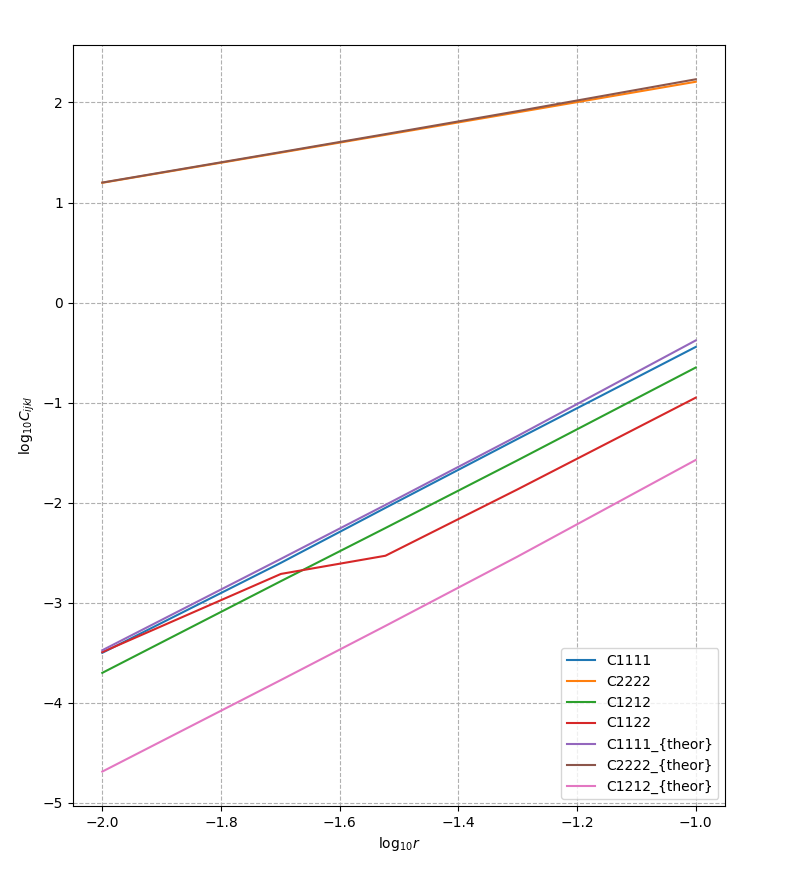
\includegraphics[width=0.8\linewidth]{img/Abaqus_CDP2.png}
    \end{center}
    \caption{La dépendance logarithmique de $r$}
\end{figure}

Remarque. On voit que $C_{2222} = const * r$. Cette relation est très proche au comportement de la famille des poutres de Bernoulli-Euler.  

\section{Annexe}

Pour la première façon on a obtenu les chiffres suivants 
\begin{table}[H]
    \begin{tabular}{|l|l|l|l|l|l|}
    \hline
     r&  0.1   &  0.05 &  0.03     &  0.02    &  0.01 \\ \hline
     $v_1$ &  9.99018  &  9.99779 &  9.99924  &  9.99967 &  9.99992 \\ \hline
     $v_2$  &  10.0098  &  10.0022 &  10.0008  &  10.0003 &  10.0001 \\ \hline
     $\varphi$ &  0.808223 &  0.777906&  0.766469 &  0.76089 &  0.755401\\ \hline
    \end{tabular}
    \caption{Les valeurs optimales après la minimisation de l'énergie pour le cas des cisaillements de la première façon}
\end{table}

Pour la deuxième façon on a reçu les mêmes résultats numériques que et pour la première façon, mais la théorie donne les valeurs différents.

\begin{table}[H]
    \begin{tabular}{|l|l|l|l|l|l|}
    \hline
     r &    0.1       &   0.05       &     0.03       &   0.02        &    0.01         \\ \hline
     $\WE{4}_{theorie\_facon2} $ &    0.0454578 &   0.00494386 &     0.00101191 &   0.000291974 &    0.0000355497 \\ \hline
     $\WE{4}_{theorie\_facon1} $                & 0.0133727 & 0.00144118 & 0.000293965 & 0.000084677 & 0.0000102929                                                                 \\ \hline
     $\WE{4}_{numerique}$ & 0.112192    & 0.01320525  & 0.002795175  & 0.000823555  & 0.00009979875 \\ \hline
    \end{tabular}
    \caption{L'énergie de cisaillements pour la deuxième façon}
\end{table}

Il faut noter, que pour les deux approches théorétiques on perde un ordre par rapport aux résultats numériques, mais par contre les chiffres sont très proches.

\begin{table}[H]
    \begin{tabular}{|l|l|l|l|l|l|}
    \hline
    r & 0.1     & 0.05    & 0.03       & 0.02        & 0.01      \\ \hline
    $v_2$ & 0.0168168 & 0.0037976 & 0.00131448 & 0.000573017 & 0.000140535 \\ \hline
    $\varphi_2$   & 0.384508  & 0.374314& 0.37045    & 0.368561    & 0.3667    \\ \hline
    $\varphi_0$ & 0.604228  & 0.585139& 0.577939   & 0.574426    & 0.570969  \\ \hline
    $\varphi_3$ & -0.999911 & -0.964939   & -0.951652  & -0.945152   & -0.938746 \\ \hline
    \end{tabular}
    \caption{Les valeurs optimales après la minimisation de l'énergie pour le cas des cisaillements de la deuxième façon}
\end{table}


\end{document}